%#!lualatex
\documentclass[11pt,pdfa,lastpage]{MishoNote}
\title{Conventions in Sho's Grading}
\author{Sho Iwamoto}
\setotherlanguages{japanese}
\hypersetup{
  pdflang={en−US},
% pdfkeywords={Supplemental note},
  pdfauthortitle={Assistant Professor, National Sun Yat-sen University},
  pdfsubject={Notes on Sho's grading conventions},
  pdfcopyright={2023 Sho Iwamoto},
  pdfcaptionwriter={Sho Iwamoto},
  pdfcontactemail={iwamoto@g-mail.nsysu.edu.tw},
  pdfcontacturl={https://www2.nsysu.edu.tw/iwamoto/},
  pdflicenseurl={https://www2.nsysu.edu.tw/iwamoto/},
% pdfpubstatus={AO},
}

%\usepackage[inline]{enumitem}
%\usepackage{tabto}

\begin{document}%
\section*{Conventions in Sho's (Japanese-like style) Grading}


\begin{tabbing}
  \kern1.3em\=\kern1.3em\=\kern4.5em\=\kern7em\=\kill
  \JA{○}\>: correct\\
  \JA{○}\kern-0.7em \raise0.3ex\hbox{\small\textsf s}\>: correct but mishandling of significant figures.\\
  \JA{×}\>: incorrect\\
  \JA{△}\>: partial mark (with a number $n$ $\to$ $n$\JA{折})\footnotemark.\\[.5em]
  \textsf{ACCEPT}: a problematic answer but accepted as a correct answer.\\[1em]


  \fbox{\makebox[1.8em]{\textsf{UM}}}\>\>: unit missing\\
  \fbox{\makebox[1.8em]{\textsf{UE}}}\>\>: unit handling error\\
  \fbox{\makebox[1.8em]{\textsf{UD}}}\>\>: unit duplication\\
  \fbox{\makebox[1.8em]{\textsf{DM}}}\>\>: direction missing\\
  \fbox{\makebox[1.8em]{\textsf{DE}}}\>\>: direction error\\
  \fbox{\makebox[1.8em]{\textsf{Dir}}}\>\>: direction missing/error\\
  \fbox{\makebox[1.8em]{\textsf{VE}}}\>\>: vector handling error\\
  \fbox{\makebox[1.8em]{\textsf{Exp}}}\>\>: insufficient explanation\\
  \fbox{\makebox[1.8em]{\textsf{Calc}}}\>\>: calculation error\\[1em]

  underline ending with \JA{┘}\>\>\>\>: correct claim for partial mark\\
  underline ending with a number\>\>\>\>: correct claim for partial mark indicated by the number\\
  underline ending with \JA{×}\>\>\>\>: incorrect claim\\[1em]

  wavy underline\>\>\>: critical issue (usually it leads you to a wrong answer)\\
  purple marker\>\>\>: English issue (tolerated)\\
  yellow marker\>\>\>: minor issue (tolerated)\\
\end{tabbing}

\vspace{3em}

\begin{DownPara}
  (Sample: For a two-second free fall of a 5\,kg object, find the final kinetic energy and the average speed.)\\
  \fbox{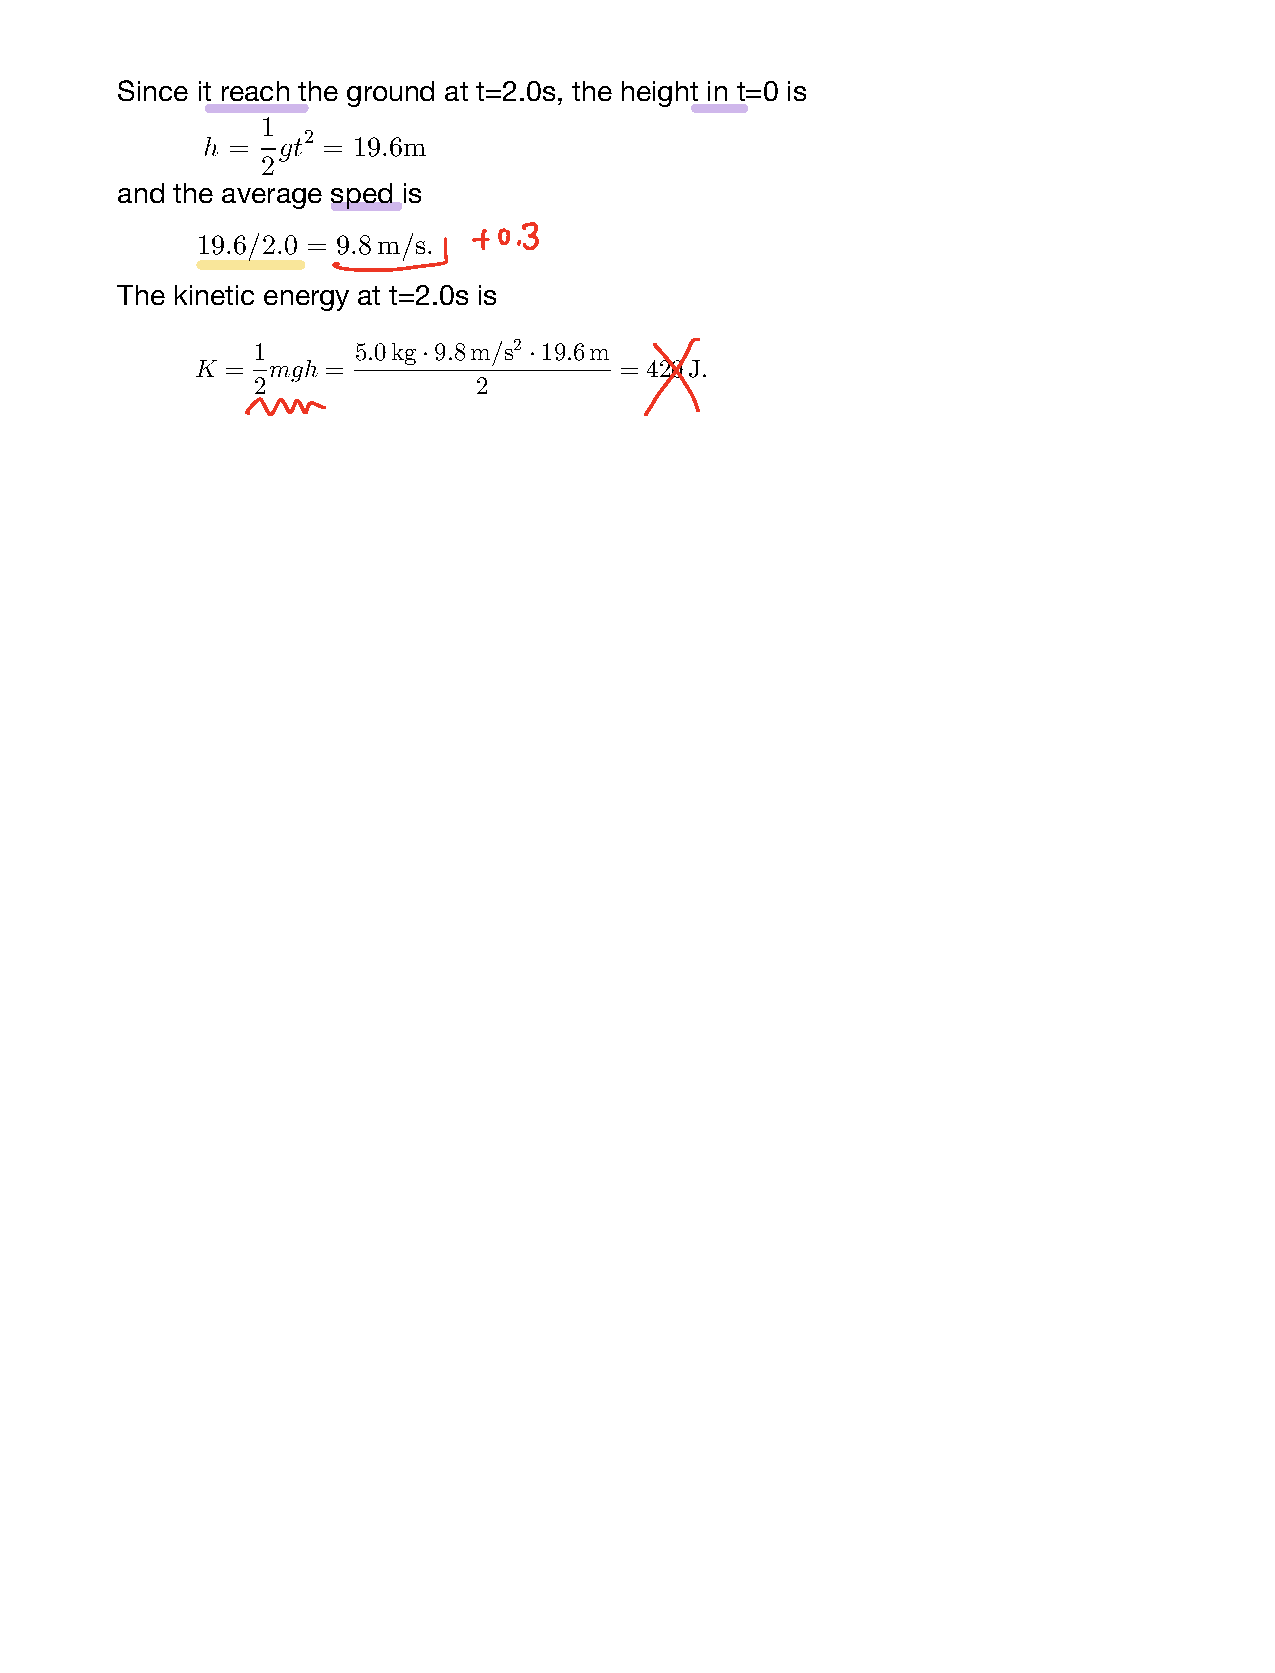
\includegraphics[width=0.6\textwidth]{grading_example.pdf}}
\end{DownPara}

\footnotetext{For $1\le n\le 9$, $\text{(full mark)}\times0.1n$. For $10\le n\le99$, $\text{(full mark)}\times0.01n$.}


\end{document}

